\input tex/hdr


Nuclear energy stemming from advanced small modular reactor (SMR) designs
holds promise as a reliable carbon-free resource capable of meeting our
nation's and the world's energy needs.  A wave of investment over the past
several years has spurred innovation in new SMR designs.
The U.S. is home to over 60 private sector advanced nuclear projects \cite{third_way},
with reactor concepts including a passively-safe Light Water SMR from NuScale \cite{nuscale},
a Salt Pebble Bed Reactor from Kairos \cite{kairos},
and a Sodium Fast Reactor (SFR) coupled with energy storage from Terrapower,
a company co-founded by Bill Gates \cite{natrium}. Recent growth in nuclear's private
sector represents an important trend as academic research projects mature
toward commercialization.

The design, certification, and licensing of novel reactor designs pose
formidable hurdles to the successful deployment of such technologies.
The lack of integral-effect test facilities for a wide range of scenarios and
conditions considered in risk-informed analysis leads to a severe deficit of
directly relevant data for these advanced designs.  Development of  appropriate
models for full-system analysis will require {\em high-fidelity numerical
simulations} coupled with advanced instrumented separate-effect experiments to
lay the ground work for subsequent integral-effect tests, when the related
facilities investment is justified.

%%%%%%%%%%%%%%%%%%%%%%%%%%%%%%%%%%%%%%%%%%%%%%%%%%%%%%%%%%%%%%%%%%%%%%%%%%
\begin{figure}[!ht]
\centering
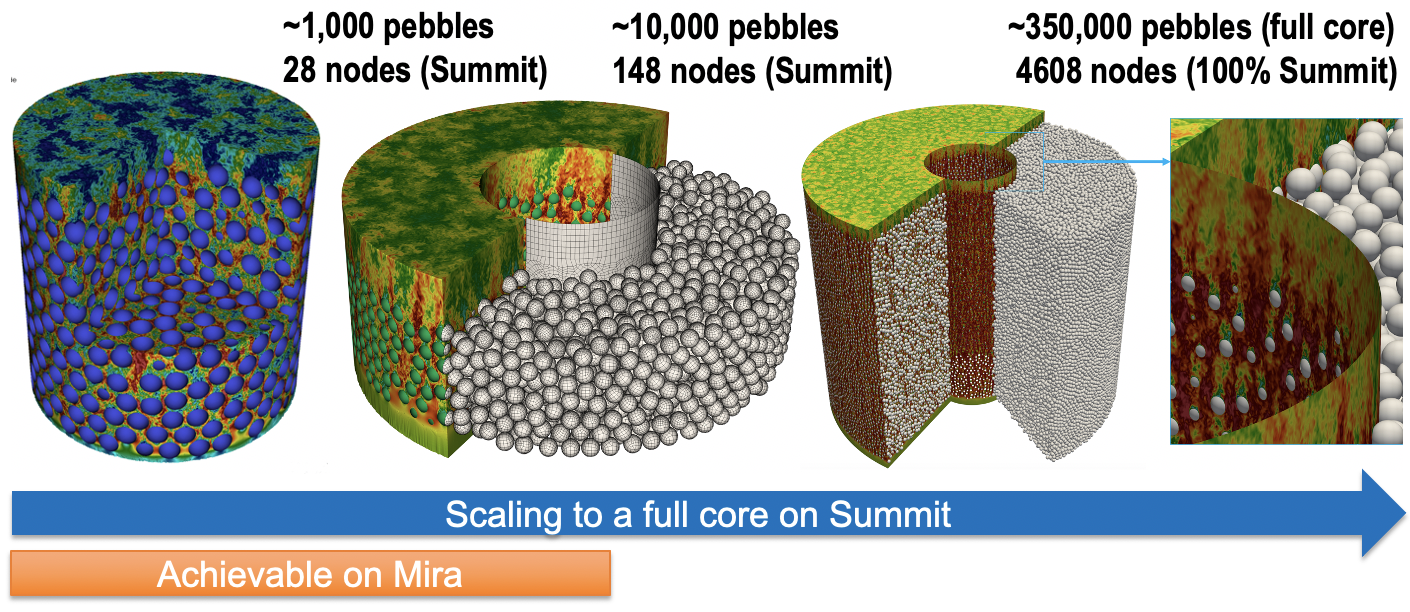
\includegraphics[width=0.93\textwidth]{figs/pebble01.png}
 \caption{\label{fig:350k} 
\small High fidelity reactor simulations of turbulent flow performed on OLCF/Summit,
enabled through DOE/NEAMS, ECP/ExaSMR and ECP/CEED collaborations:  
up to a full pebble bed core with 352,625 pebbles using an all-hex mesh comprising 
$E$=98,782,067 spectral elements of order $N=8$.
We emphasize the difference in size enabled by Summit versus Mira.}
\end{figure}
%%%%%%%%%%%%%%%%%%%%%%%%%%%%%%%%%%%%%%%%%%%%%%%%%%%%%%%%%%%%%%%%%%%%%%%%%%

Our objective is to provide the high-fidelity simulation capabilities that are
essential to this mission.  As part of this proposal, we consider SFRs and Light Water SMRs.
Both of these designs have received considerable
attention in recent years. The cores of such reactors comprise tens of
thousands of fueled rods, grouped in bundles of hundreds of rods. Coolant flow,
which is the central energy-transfer mechanism between the fissioning fuel and
electricity-generating turbines, is established between the rods to remove heat
from the nuclear fuel.  Understanding of such fluid flow over a range of
conditions is a major priority and challenge in reactor design and engineering.
Given the scale of the problem (flow in tens of thousands of channels at high
Reynolds number\footnote{The Reynolds number is a non-dimensional measure of flow
speed; high Reynolds number flows are generally turbulent, which makes them
challenging to simulate.}), the
applicability of turbulence-resolving techniques has been limited to small
portions of the reactor core. Significant compromises in accuracy have had to
be accepted in order to perform simulations at the {\em full-core} scale.
These computational economies have implications on the understanding of safety
margins, which ultimately limit economic viability, but also have broader impact
on design constraints that are harder to quantify directly.

The advent of pre-exascale supercomputers, coupled with extensive collaborations
supported through the DOE NEAMS, Applied Math Research, and ECP ExaSMR and CEED
projects, has made possible the simulation
of full reactor cores at moderate Reynolds numbers \cite{Fang2021}.  An example
is illustrated in Figure~\ref{fig:350k} for a pebble bed core, emphasizing the
difference in size enabled by recent pre-exascale architectures versus the
previous generation of supercomputers.
This proposal seeks to build on these recent achievements to develop a deeper
understanding of core-wide thermal-fluid phenomena.
\vspace*{-.1in}

\begin{displayquote}
{\it
To accelerate the deployment of SMRs and advanced reactors, this project will
use NekRS~\cite{nekrs}, the GPU-oriented version of Nek5000, to establish a full-core Large Eddy
Simulation (LES) database to support development of low-fidelity models.  
The simulations are aimed at providing critical understanding and model
development for core-wide phenomena.  The effort will take place over three
years on the supercomputers Summit and Frontier.
}
\end{displayquote}

\noindent NekRS is developed under the ECP CEED project, targeting exascale platforms.
NekRS is particularly performant on current generation GPUs such as the NVIDIA
V100s and A100s and AMD MI100s (see Table~\ref{singlerod}).  With recent
algorithmic developments, it is possible to perform a single flow-through time
for LES of a full core (Fig. 1, right) in just six hours using 27684 V100s on
Summit~\cite{peb21}.\\
\\
Our prior work in this area has led to deployment of Nek5000/RS within the
nuclear industry at vendors such as NuScale, Kairos, and Terrapower.
Nek5000 has been adopted by the Nuclear Regulatory Commission (NRC), the
organization tasked with licensing reactors for commercial use,
for purposes in the licensing process for thermal-fluid analysis.

\vspace{-.25in} \subsection{The Challenge Problems}
\vspace{-.2in}

Thermal-fluid modeling of nuclear reactors is used to predict the
proximity of the nuclear fuel to various design limits that can affect
personnel radiation dose; the ability of power conversion equipment to reliably
cool the core under a range of normal and degraded/failed equipment conditions;
and the economic viability of new operating paradigms, such as load following.
The accuracy of such simulations has direct implications on design
certification, licensing, and eventual market share.

The range of scales involved in the simulation of light water SMRs and SFRs,
and in general of rodded cores, is shown in Figure~\ref{fig:smr1} -- the range
can easily span 6 to 8 orders of magnitude, from the micrometers involved in
turbulent dissipation to meters, posing a formidable challenge.  Computational
Fluid Dynamics (CFD) is used widely in reactor design and safety analysis, but
the computational power required to resolve all relevant scales for a full-core
simulation has typically limited such geometries to less than 1\% of the core
-- usually, a single ``fuel bundle,'' or grouping of rods
\cite{wang2020,fanning,wang2020b}.  The power and flow distributions in a
reactor can be highly nonuniform, and many physics phenomena cannot be
accurately predicted with single-bundle models. Models that account for
inter-bundle coupling across the entire core are required.

%%%%%%%%%%%%%%%%%%%%%%%%%%%%%%%%%%%%%%%%%%%%%%%%%%%%%%%%%%%%%%%%%%%%%%%%%%
\begin{figure}[!ht]
\centering
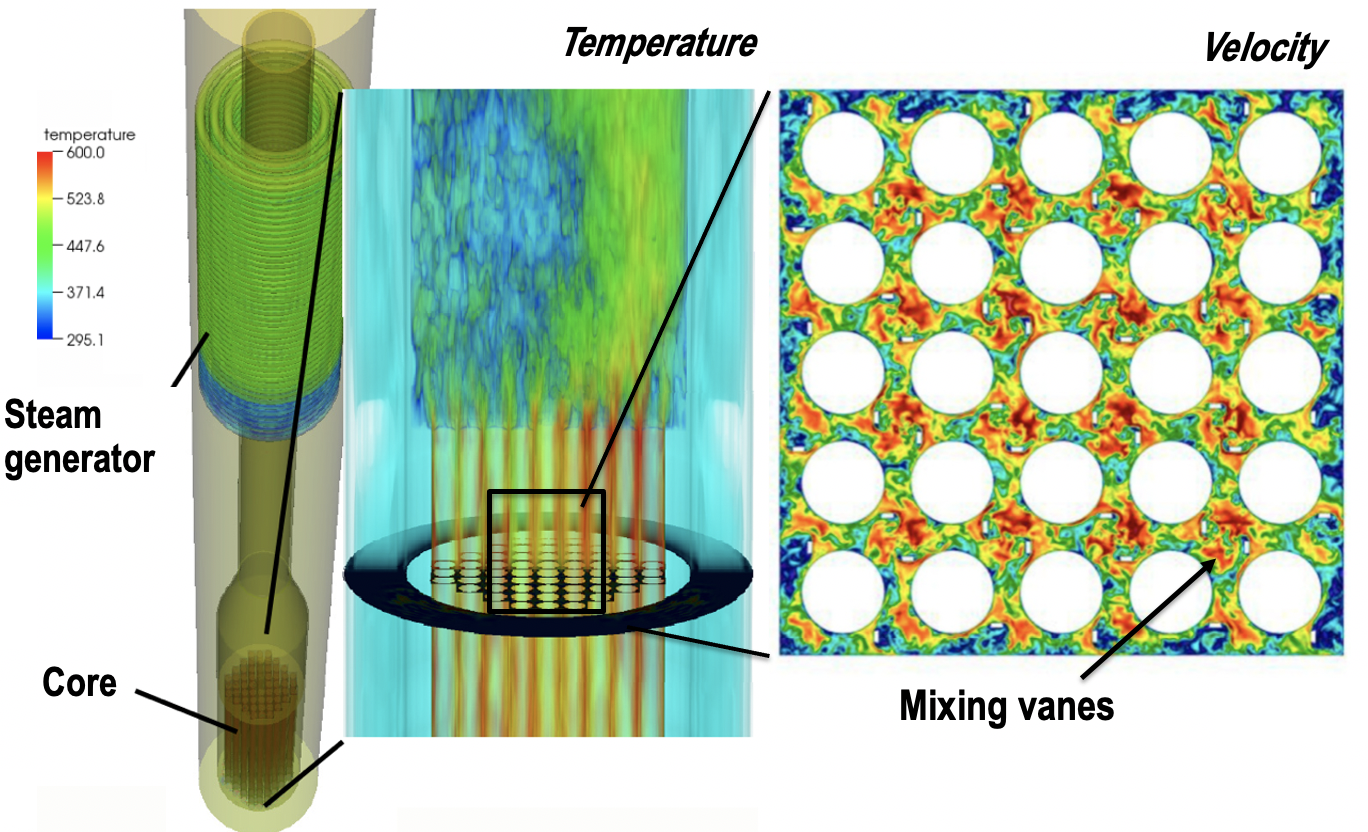
\includegraphics[width=0.9\textwidth]{figs/smr01.png}
 \caption{\label{fig:smr1}\small
Range of scales in the simulation of an SMR spanning from the full reactor
(meters, left) to turbulent dissipation (micrometers, right) generated in the
wake of mixing vanes.
} \end{figure}
%%%%%%%%%%%%%%%%%%%%%%%%%%%%%%%%%%%%%%%%%%%%%%%%%%%%%%%%%%%%%%%%%%%%%%%%%%

However, the
scale of full-core CFD has traditionally precluded its use as an analysis tool
in industry. Design teams instead rely on multiscale bridging from single-bundle
experiments/CFD models to low-cost, lower-resolution methods.
These single-bundle experiments/simulations are {\it isolated} from
the full-core physics via insulated or symmetry boundary conditions, and then used
to predict bulk heat and mass transfer corrections in the lower-resolution methods.
  Examples of coarse-mesh methods combined with CFD include the
homogenized porous media method \cite{wang2020c,Kim2020}; the ``subchannel'' method, a
finite volume method specialized to rod-type nuclear fuels \cite{blyth}; and
momentum source models \cite{hu2013}.

By nature of the scale decoupling between the CFD domain and the full core, a
key outstanding issue with this analysis approach is an inability to reliably
account for {\it interaction between global and local scales}. This recognized
limitation increases reliance on approximate methods, which in turn further
constrains the reactor design.

Light Water SMRs and SFRs both exhibit significant full-core thermal-fluid
physics for which the available low-resolution analysis methods cannot capture
important local/global interactions. In Light Water SMRs, inter-bundle mixing
due to variations in mass flow rate between assemblies as well as three-dimensional non-axial components
of the velocity (induced for example by ``LOCA holes'' \cite{jacques1997flow}) influence directly flow induced vibration (FIV) and related fuel failures.
Furthermore, the flow distribution plays an important role in the deposition of coolant contaminants on heat transfer
surfaces \cite{petrov2016prediction}. Thanks to the rapid
development of cutting-edge supercomputers, the pin-resolved CFD investigation
for an entire SMR core has been recently achieved by our team \cite{Fang2021}.
A set of momentum sources was developed to account for the effects of mixing
spacer grids while the RANS approach was applied to model the turbulence.

The first challenge problem addressed here is to further increase the simulation
fidelity of full-core SMR LES simulations by
 explicitly modeling the mixing vanes\footnote{Mixing vanes are small structures that induce coolant mixing in the core.}.
 The resulting datasets will provide the basis needed to better understand the impact of three-dimensional effects, non-homogenous flow distribution and inter-assembly mixing and improve the performance of lower fidelity models typically used in modeling the core at the design stage. This increased accuracy will translate to an uncertainty reduction and a consequent reduction in margins and better economics. We emphasize that a complete picture of three-dimensional core-wide flows is nearly impossible to obtain with experiments alone, due to the scales involved, or even through operational data, due to the lack of adequate instrumentation in actual reactors. 

In SFRs, a critical reactor design consideration is the structural expansion of
the solid fuel components in response to differential temperature and
irradiation damage gradients. The ducted fuel bundles bend and deform,
contacting neighboring bundles and transferring loads across the entire core to
restraint rings welded to the reactor vessel. These changes in core geometry
play an important role in reactor criticality (passive control) and mechanical
refueling operations.  An incomplete understanding of the structural
deformation of SFRs, especially the thermal-flow physics, has resulted in fuel
melting \cite{brittan}, rapid surges in power \cite{chaumont}, and difficulty
refueling \cite{shields} in several SFRs operated around the world.

For neutronic purposes related to transmutation and shielding, neighboring
bundles in SFRs can vary by up to a factor of 100 in power and a factor of 50 in mass
flowrate \cite{abr}. An important driver of structural
expansion in SFRs is heat transfer both within bundles and across thin gaps
between adjacent bundles that contain laminar sodium flow, a heat transfer
mechanism referred to as ``inter-assembly'' heat transfer. Even though
inter-assembly heat transfer is driven by these vastly different flow regimes
(laminar, transitional, and turbulent),
cross-bundle thermal gradients, and gap sodium flow, industry models for
core thermal-fluids are based on closures obtained from experiments and CFD
models of isolated fuel bundles without consideration of
full-core effects and realistic boundary conditions \cite{touran}.

Further, despite the fact that inter-assembly heat transfer is a major contributor
to the structural behavior of SFR cores, most industry approaches to full-core
analysis neglect the
gap flow entirely \cite{touran}, homogenize the flow into other structural
materials \cite{fiorina_of}, or neglect certain azimuthal heat transfer
paths between neighboring bundles \cite{touran} -- without correction terms to account for the
un-resolved physics \cite{touran,fiorina_of}. Some researchers substitute Reynolds
Averaged Navier-Stokes (RANS) CFD for small regions in a full-core low-resolution
model \cite{wang2020,gerschenfeld,Kim2020}, an approach that is still subject to
 reduced accuracy compared to resolved CFD simulations.

The nuclear industry has an acute need for LES-informed models for
inter-assembly heat transfer -- no models exist for inter-assembly heat
transfer considering the coupling between global and local effects. Common
approximations for local heat transfer do not fully characterize this
global heat transfer mechanism, and this knowledge gap
may result in significant
underprediction of heat removal \cite{gerschenfeld}, requiring over-engineered
safety systems or sub-optimal power density. Therefore, the second challenge
problem addressed here is to develop inter-assembly heat transfer models with
full-core LES that properly account for the interaction between flow regime and
power distributions on core-wide fission heat redistribution.

%{\bf TODO: What other content should go here? Maybe more discussion of typical
%problem sizes people have done before? Typical DOFs for a full-core porous
%media/subchannel solve? Resolution comparison?}

%{\bf Talk about why Petascale resources are required}
%Petascale resources are required to understand how the interactions between
%laminar, mixed convection, and forced convection flow regimes affect
%inter-assembly heat transfer.

%Explain what advances you expect to be enabled by an INCITE award that
%justifies an allocation of petascale resources (e.g., anticipated impact on
%community paradigms, valuable insights into or solving a long-standing
%challenge, etc.).

% Place the proposed research in the context of competing work in your
% discipline or business.

% State clearly the challenge problem or problems we are trying to solve.  Make
% clear statements about impact.

\vspace{-.25in}
\subsection{Impact and Insights}
\vspace{-.2in}

This proposal aims to provide insights into two grand challenges in the design
of rod-type nuclear reactors by developing an LES database to support the
development of lower fidelity models.  The first is directed at SMRs, the
second at SFRs.
Both grand challenges share the same
motivating gap analysis -- reduced-geometry CFD models cannot properly account
for the interaction between core-wide physics and local thermal-fluids. By
developing more accurate lower fidelity models informed by turbulence-resolved
CFD, this proposal seeks to reduce risk to the technical design, economic
viability, and licensing of advanced reactor concepts.

The reactor development timeline, from conception to power generation, often
takes decades to accomplish; much of the reactor design and analysis is
``front-loaded'' to allow sufficient time for the licensing process, a
prerequisite to construction. The two challenge problems selected in this
proposal will have immediate technical and business impact to the nuclear
industry by coinciding with large Light Water SMR and SFR development programs
in private industry and the DOE.

% feel to add some statements that can further highlight the business impact
Several strategically important projects have been identified and are being pursued by
the Exascale Computing Project (ECP) for the upcoming exascale computing platforms.
Among these, the ExaSMR project is specifically focused on SMRs.
SMRs offer the prospect of affordable baseload electricity production while
avoiding some of the traditional limitations that encumber large reactor designs,
such as high capital costs and long construction timelines.
As a result, government, industry, and academia have all expressed interest in
SMR research and development.
The objective of the ExaSMR project is to use exascale computing platforms to
carry out extreme-fidelity multi-physics simulations of SMRs, namely,
to enable verification and validation of current analysis methods by
generating detailed power distributions during startup conditions,
full-cycle depletion analysis, and fast transient behavior characteristics of
accident scenarios \cite{Merzari2018}.
Significant progress has been made in both the coupling of Monte Carlo (MC) neutronics
and CFD \cite{Hamilton2018,Hamilton2019} and the development of CFD modeling
capabilities \cite{Fang2021,Merzari2018}. Our emphasis on high-resolution
LES modeling of SMRs will complement these efforts.

As part of the DOE, the Advanced Reactor Demonstration
Program (ARDP) awarded TerraPower, a private nuclear development company
co-founded by Bill Gates, funds
to develop and build an advanced SFR by 2027 \cite{ardp_tp}. The next two to
three years are the opportune moment for the LCF to have an impact on the
viability of this SFR design by making available to industry more accurate
inter-assembly heat transfer models. The thermal-fluid physics is the most important
contributor to transient structural deformation in SFRs \cite{wozniak}, and
structural deformation measurements often have the highest uncertainty among a number of
other important core phenomena \cite{lum}.

Limited experimental data exists for inter-bundle mixing in Light Water SMRs
and for inter-assembly heat transfer in SFRs, necessitating greater reliance on
modeling and simulation. There
are therefore significant potential business impacts to the success of this
research, such as 1)~reduced calculation uncertainty that enables operation closer
to thermal and irradiation limits; 2)~simplified reactivity control mechanisms;
and 3)~improved predictive maintenance capabilities.
As the U.S.'s nuclear plant construction
experience has waned over the past decade \cite{schlissel}, the viability of
nuclear power in a clean energy portfolio depends on reducing cost through
uncertainty reductions and design simplifications such as the above.

In addition to direct impacts in the nuclear industry, this research will spur
a paradigm shift in high-resolution modeling of nuclear systems. Competing work
in our field remains directed at the single-bundle level both in CFD
simulations \cite{wang2020,fanning,wang2020b,Boyd2016} and experiments
\cite{Nguyen2017,Bhowmik2021,goth,song_2020,martin2020}.
Only LCF resources are viable for the proposed full-core LES simulations
-- our simulations will be approximately 1000\(\times\) the size of current
``state-of-the-art'' experiments and CFD simulations performed by other groups.
Our full-core simulations will be first-of-a-kind in addressing core-wide reactor thermal-fluids and build upon
our group's previous works \cite{Fang2021}, helping ushering in a new era where such simulations are possible.

%The success of this research will
%change the notion
%that rod-resolved, full-core CFD is still 5\(+\) years away.

% Elia: I COMMENTED THIS OUT BECAUSE I DO NOT THINK IT IS A STRONG ARGUMENT. THE PROPOSAL HAS ITSELF A TIMELINE OF 3 years? April: good point

% anticipated impact on community paradigms, valuable insights into or solving
% a long-standing challenge, etc.).

\vspace{-.25in}
\subsection{Previous INCITE Awards}
\vspace{-.2in}

The PI has not received any INCITE award and no previous INCITE award is directly related to the outlined project.

\vspace{-.25in}
\section{RESEARCH OBJECTIVE AND MILESTONES} % typically about 6 pages
\vspace{-.2in}

% Describe the proposed research, including its goals and milestones and the
% theoretical and computational methods it employs. Goals and milestones should
% articulate simulation and developmental objectives and be sufficiently
% detailed to assess the progress of the project for each year of any
% allocation granted.  Milestones should correlate with those in Section 4,
% “Milestone Table.”
% It is especially important that you provide clear connections between the
% project’s overarching milestones, the planned production simulations, and the
% compute time expected to be required for these simulations (e.g., should
% correlate with Section 2.3.i, “Use of Resources Requested”) in the research
% proposal.  You should also make clear any dependencies of milestones on other
% milestones.

In the past ten years, the Nuclear Energy Advanced Modeling and Simulation
(NEAMS) program \cite{sofu2017us} has invested in developing modern advanced
CFD software to facilitate the deployment of advanced reactors. In fact, CFD is
currently in widespread use both in reactor design and in safety analysis, as
testified by the increasing number of articles in the field. Among recent
examples, Roelofs \cite{roelofs2018thermal} illustrates the importance of CFD
to liquid metal reactor design and analysis. Detailed modeling and simulation
is of particular importance for advanced reactors, where simulation can be used
in conjunction with separate effect experiments, in the absence of extensive
integral test data (at least in the initial phases of development).

RANS \cite{conner2010cfd} and occasionally Unsteady Reynolds Averaged
Navier-Stokes (URANS) remain the workhorses for analysis conducted in industry,
research centers, and academia.  However, despite significant advancements in
turbulence modeling in recent years, RANS is limited in terms of accuracy.
Turbulence modeling remains a source of uncertainty in complex engineering
flows, as RANS models are not general and are sensitive to even small geometric
changes \cite{merzari2010numerical}. Moreover, RANS and URANS remain limited in
predicting turbulent fluctuations and high order statistics which may be of
interest in important applications such as FIV and
FSI \cite{yuan2017flow}.

In contrast to RANS, wall-resolved LES and Direct Numerical Simulation (DNS)
have a much lower degree of uncertainty and can provide valuable and
unprecedented insight into the flow physics. Historically, however, these
methods have been limited to small geometries, such as sub-channels
\cite{grotzbach1999direct}, due to the high computational cost associated with
both techniques. From the late 1990s to the end of the 2000s, LES/DNS remained
a niche application for nuclear engineering flows. The review of Grotzbach
\cite{grotzbach1999direct} provides a comprehensive status of the capabilities
available in that time frame. Toward the end of the 2000s however, larger scale
calculations started to emerge \cite{pointer2009simulations}.

In fact, since the advent of petascale computing (i.e, computers
capable of more than 1 petaflop), the simulation of portions of nuclear
components has been demonstrated with LES \cite{merzari2017large}.
For example, some landmark calculations conducted with Nek5000/RS are presented in
Figure~\ref{f:examples}. The advent of pre-exascale machines has enabled the simulation of larger systems including a full core SMR \cite{Fang2021}.

\begin{figure}[!ht]
\centering
\includegraphics[width=0.93\textwidth]{figs/examples.png}
%\includegraphics[width=0.93\textwidth]{figs/examples.png}
\caption{\small Examples of large-scale LES/DNS simulation of nuclear reactor flows.
a-b) Cross sections of the flow in helical coil steam generator
\cite{alper2018}; c) Velocity magnitude in a 61-pin wire-wrapped rod bundle
\cite{goth2018comparison}; d) Velocity magnitude in a random pebble bed
\cite{yuan2019}.} \label{f:examples}
\end{figure}

% add more of a description of the proposed research and its goals

\begin{displayquote}
\textit{
Building upon the extensive experience of our group and recent achievements, this proposal seeks the development of a set of full-core LES
datasets to address knowledge gaps in inter-assembly heat and mass
transfer in nuclear reactors.
}
\end{displayquote}

\vspace{-.25in}
\subsection{Theoretical and Computational Methods}
\vspace{-.2in}

We consider the velocity, continuity, and energy equations that
describe the constant-property incompressible flow of a Newtonian fluid in the
absence of other body or external forces:
\begin{equation}
\frac{\partial  u_i  }{\partial t} +  \frac{\partial}{\partial x_j} \left( u_i u_j \right) =-\frac{1}{\rho} \frac{\partial p}{\partial x_i} + \frac{\partial}{\partial x_j} \left[ \nu \left( \frac{\partial u_i}{\partial x_j} +\frac{\partial u_j}{\partial x_i} \right) \right]
\label{eq:UEqn}
\end{equation}
\begin{equation}
\frac{\partial u_i}{\partial x_i} = 0
\label{eq:rhoEqn}
\end{equation}
\begin{equation}
\rho c_p \left( \frac{\partial T }{\partial t} + u_j \frac{\partial T}{\partial x_j} \right) = \frac{\partial }{\partial x_j} \left( \lambda \frac{\partial T}{\partial x_j} \right)
\label{eq:EEqn}
\end{equation}
where $u$ is the velocity, $p$ is the pressure, $T$ is the temperature, $\rho$
is the  density, $\nu$ is the kinematic viscosity, $\lambda$ is
the thermal conductivity, and $c_p$ is the heat capacity. In natural
convection cases, the Boussinesq or low Mach approximations
\cite{tomboulides1997numerical} are applied, leading to different
formulations available in Nek5000/RS.
{\it Nek5000/RS is the primary code that will be employed
in this analysis.}

We restrict our discussion to turbulence-resolving simulations such as DNS and
wall-resolved LES. In advection-dominated problems such as the one described by
Eqs. (\ref{eq:UEqn})--(\ref{eq:EEqn}) at moderate to high Reynolds numbers, the
high-wavenumber component of transported quantities does not decay
exponentially, as observed in diffusion-dominated problems. Therefore, both
meaningful signals and numerical errors can persist in time, and appropriate
numerical schemes must be selected in order to avoid excessive dispersion.
The spectral element method, which is the basis for Nek5000/RS, is ideally
suited for this type of analysis. We note that LES is usually performed within
Nek5000/RS using an explicit filter \cite{schlatter21}.

\vspace{-.25in}
\subsection{Description of Tasks}
\label{sec:tasks}
\vspace{-.2in}

% goals and milestones should articulate simulation and developmental
% objectives and be sufficiently detailed to assess the progress of the project
% for each year

The overarching goals of this proposal are twofold.  First, to develop
reference full-core LES CFD predictions that will be compared against
lower-resolution models to {\it provide unprecedented insight into the
interaction between global and local thermal-fluid effects} for rod bundle
nuclear reactors. The second is to {\it develop a full-core LES CFD
database to inform low-resolution methods}. Each of these goals are now
detailed in terms of major tasks for each of the challenge problems.

\vspace{-.25in}
\subsubsection{Light Water Small Modular Reactor (SMR) Challenge Problem}
\vspace{-.2in}

To address the SMR challenge problem of assessing three-dimensional core-wide
flow and heat transfer behavior we examine an extension of the work of Fang et
al. \cite{Fang2021}.  In this previous work we have modeled with RANS and
momentum sources an SMR core comprised of 37 assemblies (each 17$\times 17$),
inspired by the Nuscale core. Each assembly has an active fuel length of $2$ m
for which the power distribution is obtained with a precursor Monte Carlo
neutron transport calculation. The Reynolds number based on the rod diameter
and the bulk velocity is $Re=50000$ and the Prandtl number is $Pr=1$.

We now propose to gradually increase the resolution of the simulations by
modeling an increasing number of assemblies with higher resolution using a
zonal LES approach on Summit \cite{menter2012global}. The mixing vanes in the
higher resolution assemblies will be meshed in detail (explicitly modeled)
and turbulence will be
resolved using LES. At later stages in the proposed research, we propose to
model the entire core with LES on Frontier. This gradual approach will allow us
to make maximum use of available resources (i.e., LES with mixing vanes is
currently impossible on Summit) and will also allow identification of the
number of detailed assemblies needed to accurately account for the flow within
a target assembly within the context of a zonal LES simulation. The major tasks
have been identified as follows:

\vspace{-.15in}
\begin{enumerate}[label=\textbf{\Roman*}]
\item Develop full-core RANS mesh with one assembly explicitly modeled using
LES.  Perform mesh convergence studies for a single LES bundle. Conduct CFD
simulations and extract relevant information on flow spectra and mixing at the
interface between the resolved (LES) and RANS assemblies.
\item Develop a full-core RANS mesh with nine assemblies explicitly modeled. Conduct CFD simulations and extract relevant information on flow spectra and mixing at the interface 
between the resolved and RANS assemblies.
\item Develop full-core LES mesh with all assemblies explicitly modeled.
Conduct CFD simulation. Extract relevant information on flow spectra and 
inter-bundle mixing at the interface between assemblies. Perform averaging and
characterize flow distribution across the full core.
\end{enumerate}
\vspace{-.15in}

This work will answer several outstanding questions:

\vspace{-.15in}
\begin{itemize}
\item How does inter-bundle mixing affect core temperatures? Temperatures correlate with deposition of coolant contaminants on the fuel heat transfer surface.
\item How does the mixing vane impact momentum losses and inter-bundle mixing? Trade-offs between pressure loss and enhanced mixing may illuminate new insights into nuclear fuel design.
\end{itemize}
\vspace{-.15in}

The above questions will be addressed by comparing temperature, pressure, and mass flux distributions across the LES database.

% {\bf Is it worth mentioning what system we're modeling? I call out ABR in the
% next section. Either let's do the same here or cut out the ABR specifics in the
% next section}

\vspace{-.25in}
\subsubsection{Sodium Fast Reactor (SFR) Challenge Problem}
\vspace{-.2in}

To address the SFR challenge problem of inter-assembly heat transfer, full-core
LES CFD simulations will be conducted for the Advanced Burner Reactor (ABR), an
open-source reactor design that is considered a prototype of a large commercial
SFR \cite{abr}. The objectives of these simulations are to 1)~answer
outstanding questions about the nature of inter-assembly flow and heat transfer
and 2)~utilize the produced LES database to generate bulk heat
transfer correlations to improve the predictive capabilities of
lower-resolution tools. The major tasks have been identified as follows:

\vspace{-.15in}
\begin{enumerate}[label=\textbf{\Roman*}]
\item Develop full-core meshes and test at scale to ensure high quality. Mesh
    convergence studies will be conducted for small groups of bundles under a
    variety of power and flow gradients to establish applicability to full-core
    geometries. 
\item Develop low-resolution full-core models using the NEAMS
    porous media application, Pronghorn \cite{novak2021b}. These models will be
    compared against the generated LES database to assess the effect if proper
    resolution of global/local physics interactions. Low-resolution models will be
    run with non-LCF computing resources, including the {\em Nek5000} cluster in
    ANL's Nuclear Engineering Division.
\item Conduct full-core LES CFD simulations of the ABR at three power-to-flow
  ratios\footnote{The ``power-to-flow'' ratio is a measure of the relative
  balance between core power and core cooling. A power-to-flow ratio of unity
  indicates nominal operating conditions.} that may be observed during actual
  operation. These conditions correspond to full power (1000 MWth) and a)~nominal
  flow (\(Re=90000\)), b)~moderately reduced flow (\(Re=72000\)), and
  c)~significantly reduced flow (\(Re=60000\)). A fourth condition at decay heat
  removal conditions (\(Re=650\) and 7.5 MWth) will also be included to cover the
  very low range in power-to-flow ratio.  
\item Compare LES database with
  reference low-resolution models developed in Task II. Evaluate the physics
  consequence of industry modeling simplifications to inter-assembly heat
  transfer.  
\item Post-process LES database to generate an effective thermal
  conductivity model applicable to subchannel and porous media methods. Apply new
  closure to the models developed in Task II and quantify the improvement in
  accuracy.
\end{enumerate}
\vspace{-.15in}


%% {\bf We can cut some of this if needed. Currently a lot more emphasis is placed
%% on this secondn challenge problem, when they should be more equal}
Additional details are now provided for each task. During Task I, full-core
meshes will be generated for the prototypic design. Mesh convergence will be
performed with \(h\)-type refinement\footnote{$h$-type refinement refers to
mesh convergence realized by reducing element size.} to leverage past
experience with optimal element counts per GPU on Summit. Initial RANS
simulations will be performed on Summit.  Full-core models will be constructed
for the four operating conditions (detailed in Task III) based on
openly-available material properties, power, and mass flow distributions.
During Task II, equivalent low-resolution models will be constructed and run on
workstations available to our group at ANL.


During Task III, full-core LES CFD simulations will be conducted for four
different combinations of core power and flowrate. The first condition
corresponds to the nominal reactor state. The second two conditions correspond
to power-to-flow ratios 25\% and 50\% higher than nominal conditions, which are
indicative of reactor trip points \cite{chaumont} and unmitigated equipment
failure, respectively. The last simulation corresponds to decay heat removal
after the fission reaction has been terminated.

In Task IV, the LES database will be compared against the reference low-resolution models to answer several outstanding questions: \\[-5ex]

\vspace{-.15in}
\begin{itemize}
\item How does inter-assembly heat transfer affect core temperatures? The core
      outlet temperature distribution has a direct impact on thermal stresses and
      lifetimes of downstream components.  
\\[-4.5ex]
\item How is inter-assembly heat transfer affected by the power-to-flow ratio?
      The wide variation in flow regime across the core may result in global heat
      redistributions with flowrate changes.  
\\[-4.5ex]
\item Are significant cross-flows generated across the core? In submerged
    ``pool-type'' reactor concepts, such flows could draw fluid from
    bypass regions, changing fuel temperature distributions.  
\\[-4.5ex]
\end{itemize}
\vspace{-.15in}

The above questions will be addressed by comparing temperature and mass flux
distributions across the LES database, as well as comparing temperature
distributions between the LES database and lower-resolution models. Finally, in
Task V, the LES database will be used to produce an effective conductivity
model for use in lower-resolution tools. By homogenizing over element sizes
typical of porous media models, the heat flux computed along the boundaries of
the inter-assembly region will be used to compute an effective conductivity
\(\kappa\),
\begin{equation}
q_i^{''}=-\kappa_{ij}\frac{\partial T}{\partial x_j}\ ,
\end{equation}
where \(q^{''}\) is the heat flux and \(\kappa_{ij}\) is a diagonal tensor. In other words, the mechanism by which the LES database will inform lower-resolution tools is by introducing a correction to the heat transfer in the inter-assembly space. Due to the small gap width of the inter-assembly space, Courant-Friedrichs-Lewy (CFL) limits, and ensuing time step limitations, are of paramount important to low-resolution methods. Therefore, low-resolution tools such as those used by Terrapower \cite{touran} approximate the fluid flow in the inter-assembly region as a conducting solid. By supplying a necessary closure, \(\kappa_{ij}\), for this model, the proposed research is {\it compatible with industry modeling tools} and can be rapidly integrated into the industry design process.

\vspace{-.25in}
\subsection{Milestones}
\vspace{-.2in}

% milestones should correlate with those in Section 4, Milestone Table
% provide clear connections between the project's overarching milestones, the
% planned production simulations, and the compute time expected for these
% simulations (should correlation with Section 2.3.i - use of resources
% requested).

A set of milestones has been developed to spread the computational load over
the expected 3 year term of the project; these milestones are listed in
Table~\ref{tab:milestones} and represent the tasks in Section~\ref{sec:tasks}.
The milestones in Table~\ref{tab:milestones} are directly correlated with the
Milestones (Section 4 in the submitted material), where additional information
is provided with respect to required computing resources.

\input tex/table1

% \begin{table}[h!]
% \footnotesize
% \centering
% \caption{Summary of the tasks and milestones associated with this proposal. 
% %``Low-res.'' indicates ``low-resolution.''
% }
% \begin{tabular}{c c c l l l l}
% \toprule
% Problem & Task & Milestone & Description & End Date & System & Node Hours\\
% \midrule
% \multirow{6}{*}{SMR} & \multirow{2}{*}{I} & A & Mesh and input setup (1 assembly explicit) & Jun 2022 \\
% &  & B & Zonal LES simulation (1 assembly explicit)  & Dec 2022 \\\cmidrule{2-5}
% & \multirow{2}{*}{II} & A & Mesh and input setup (9 assembly explicit)  & Jun 2023 \\
% &  & B & Zonal LES simulation (9 assembly explicit)  & Dec 2023 \\\cmidrule{2-5}
% & \multirow{2}{*}{III} & A & Mesh and input setup (LES simulation) & Jun 2024 \\
% &  & B & Full core LES simulation  & Dec 2024 \\
% \midrule
% \multirow{14}{*}{SFR} & \multirow{3}{*}{I} & A & Mesh convergence studies for clusters of bundles & May 2022 \\
% & & B & Complete full-core mesh and models & July 2022\\
% & & C & Preliminary results of full-core CFD model (RANS) & Dec 2022\\\cmidrule{2-5}
% & \multirow{3}{*}{II} & A & Complete full-core Pronghorn low-res. models & Nov 2022 \\
% & & B & Preliminary tests of full-core low-res. model & Nov 2022\\
% & & C & Full-core low-resolution simulations & Dec 2022\\\cmidrule{2-5}
% & \multirow{2}{*}{III} & A & Preliminary LES simulations  & Dec 2023\\
% & & B & Final LES simulations  & Dec 2024\\\cmidrule{2-5}
% & \multirow{2}{*}{IV} & A & Temperature measurements from LES database & Mar 2024\\
% & & B & Crossflow measurements from LES database & Jun 2024\\\cmidrule{2-5}
% & \multirow{3}{*}{V} & A & Correlate LES database with \(\kappa\) model & Sep 2024\\
% & & B & Repeat full-core low-res. simulations with new closure & Oct 2024\\
% & & C & Temperature measurements from LES database & Dec 2024\\
% \bottomrule
% \end{tabular}
% \label{tab:milestones}
% \end{table}
 
For the SMR modeling, Task I encompasses model setup and preliminary testing
for the Zonal LES CFD simulations. Our group has extensive experience with
modeling of mixing vanes \cite{busco2019invariant}; milestone I.A will develop
guidelines for converged meshes for all subsequent simulations and deliver the
first full core mesh with an assembly explicitly modeled, while milestone
I.B will deliver the simulation results.  Through tasks II and III we then
progress to the full core in later years.

For the SFR modeling, Task I encompasses model setup and preliminary testing for
the LES CFD simulations. Our group is experienced at meshing such geometries \cite{merzari2020toward}; milestone
I.A will develop guidelines for converged meshes for all subsequent simulations, while milestone
I.B will generate full-core meshes and apply realistic power and mass flow distributions to the model.
Milestone I.C will then conclude Task I by conducting RANS flow simulations. This will help ensure the resolution of the LES simulations is adequate.
During Task II, we will develop low-resolution models of the same reactor system;
due to the small computational requirements of these low-resolution models, mesh
refinement studies will be performed directly on the full core model. In Task
III, we will begin our flow simulations for the \(Re=650\) and then follow with
simulations at higher Reynolds number. This strategy will allow us to continue
gaining insights into the parallelization strategies for the flow case with the
lowest mesh resolution requirements. Task IV and V focus on the post-processing
of the data and comparisons with results from Task II. They are conducted in
parallel with Task III.

%{\bf Need to describe HERE a node hours justification for each task, and how
%the tasks differ from each other in that regard. Must match table in appendix.}
\input tex/readiness



% ....STORAGE
% ....Conversion of hours to Frontier

10 words per GLL --- 
